\section{VLSI implementation}

Lo scopo di questa sezione è quello di presentare l'implementazione del filtro IIR progettato, che nella fattispecie è un filtro IIR con precisione di 10 bit e ordine pari a 1. In \autoref{fig:filtro_generic} {\LARGE correggere} è mostrata l'interfaccia del filtro dove il parallelismo $n_b$ è fissato a 10 ed essendo l'ordine del filtro pari a 1, i coefficienti necessari sono $a_0, a_1, b_0, b_1$.

\begin{figure}[h]
	\center
	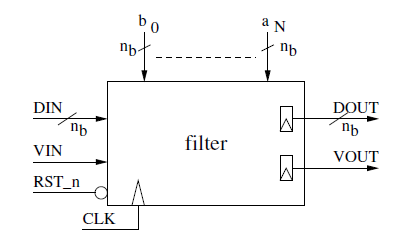
\includegraphics[width=0.4\textwidth]{filtro_generic.png}
	\caption{Filter pinout}
	\label{fig:filtro_generic}
\end{figure}


\subsection{VHDL model}
In ingresso e in uscita al filtro sono posti dei registri per sincronizzare i dati con il clock e due segnali di validazione per i dati, $VIN$ and $VOUT$. In \autoref{fig:IIR_1} è mostrata l'architettura del filtro, dove i registri sono stati trascurati, la forma utilizzata è la direct form II. I dati in ingresso campionati entrano dalla porta $x[n]$, vengono elaborati e i risultati fuoriescono dalla porta $y[n]$. Il parallelismo interno della macchina è diverso da quello esterno, per evitare la possibilità di avere overflow con qualsiasi combinazione di dati in ingresso quando viene effettuata la somma, la precisione è stata estesa a 12 bit effettuando un'estensione del segno a tutti i segnali in ingresso. La moltiplicazione invece non ha problemi di parallelismo perché si riesce ad avere una precisione sufficiente troncando i bit meno significativi ad ogni moltiplicazione e avendo quindi stesso parallelismo tra dati in ingresso e in uscita. Il registro interno alla macchina ha un segnale di enable che viene gestito dal segnale di validazione del dato in ingresso in modo che quando si ricevono dati non validi, esso non campiona mantenendo il dato in uscita corretto.

\begin{figure}[h]
	\center
	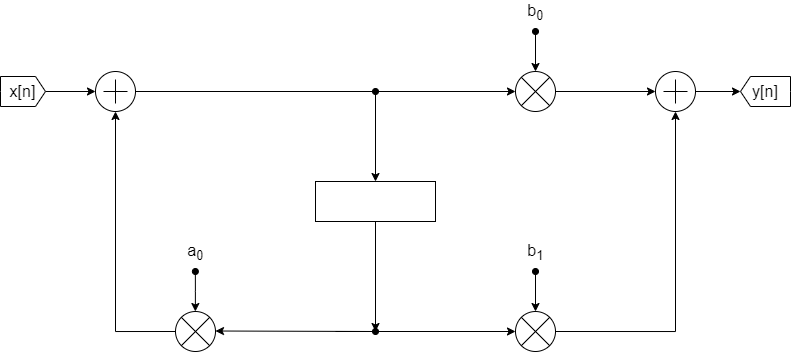
\includegraphics[width=0.8\textwidth]{iir_1.png}
	\caption{IIR filter architecture}
	\label{fig:IIR_1}
\end{figure}

\subsection{Simulation}
Per la simulazione del circuito è stata adottata una soluzione simile a quella consigliata con un generatore di dati in ingresso e un error checker in uscita. E' stato utlizzato uno script python per generare una forma d'onda sinusoidale, che viene elaborata in parallelo dal circuito da noi progettato e dall'ideal model descritto in C. I risultati in uscita sono scritti su due file che vengono elaborati da un ulteriore script python che calcola l'errore come differenza tra l'output del DUT e quello del C model.
In \autoref{fig:wave_sim} è mostrato il wave con i segnali del DUT. Si nota come quando il segnale $VIN$ diventa valido il circuito inizia a campionare i dati in ingressoe dopo una latenza di 2 colpi di clock i risultati sono pronti in uscita, infatti il segnale $VOUT$ diventa alto. Infine si nota il corretto funzionamento anche quando $VIN$ va a 0, infatti i dati all'uscita del registro di ingresso, $reg\_out$, rimangono invariati quando si verifica questa situazione sintomo che il circuito smette di campionare i dati in ingresso.

\begin{figure}[h]
	\center
	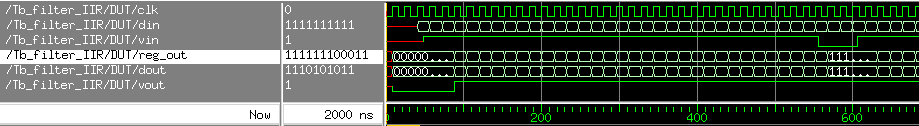
\includegraphics[width=1\textwidth]{images/wave_vin_0_1.png}
	\caption{Wave results of the simulation}
	\label{fig:wave_sim}
\end{figure}

Dopo aver verificato il corretto timing del circuito, sono stati controllati i risultati numerici prodotti. In \autoref{tab:tab_results} è mostrato un estratto dei dati in uscita dal modello ideale e dal circuito progettato a fronte dello stesso set di dati in ingresso. Si nota come ci sia una perfetta ugualianza dei risultati che conferma la correttezza di funzinamento del filtro progettato.

\begin{table}[h]
\begin{center}
\begin{tabular}{|l|l|l|l|}
\hline
Input & DUT output & C model output & Error \\
\hline
511 & 252 & 252 & 0 \\
-1 & 213 & 252 & 0 \\
414 & 207 & 207 & 0 \\
-1 & 98 & 98 & 0 \\
158 & 80 & 80 & 0 \\
-1 & -56 & -56 & 0 \\
-159 & -77 & -77 & 0 \\
-1 & -188 & -188 & 0 \\
-415 & -206 & -206 & 0 \\
-1 & -250 & -250 & 0 \\
\hline
\end{tabular}
\end{center}
\caption{Results of the simulation}
\label{tab:tab_results}
\end{table}



\subsection{Logic Synthesis}
Verificato il corretto comportamento del circuito con Modelsim si è passati alla sintesi con Synopsys. Il primo obiettivo è quello di cercare la frequenza massima che permetta il corretto funzionamento del circuito e la relativa area. Sono state sfruttate le librerie di porte standard fornite che permettono di sintetizzare in automatico anche i blocchi logici più complessi come sommatori e moltiplicatori.
In una fase preliminare è stato impostato un clock con periodo $T_{clk} = \SI{10}{\nano\second} \pm \SI{0.07}{\nano\second}$. Il risultato della sintesi mostra uno slack di $+\SI{5.14}{\nano\second}$; il fatto che lo slack sia positivo implica che i vincoli sul clock impostati sono stati rispettati con la sintesi ottenuta.
Per calcolare la frequenza massima è stato impostato in una prima fase il clock nullo, in qusto modo teoricamente lo slack negativo ottenuto dovrebbe corrispondere al minimo periodo clock necessario. Questo però non è vero, infatti impostando il clock al nuovo valore si ottiene ancora uno slack negativo. Questo comportamento è dovuto al fatto che il sintetizzatore cambia la struttura del cirucito interno in base al vincolo fornito sul clock come si nota dai dati sull'area. E' stato necessario iterare questo procedimento più volte per ottenere uno slack nullo. In \autoref{tab:timing_rep} è mostrata una sintesi dei risultati ottenuti.

\begin{table}[h]
\begin{center}
\begin{tabular}{|l|l|l|}
\hline
$T_{CLK} [ns]$ & slack [ns] & area $[(\SI{}{\micro\meter})^2]$ \\
\hline
10 & 5.14 & 1991 \\
0 & -3.13 & 2491 \\
4.10 & 0 & 2187 \\
16.4 & 11.54 & 1991 \\
\hline
\end{tabular}
\end{center}
\caption{Results of timing report}
\label{tab:timing_rep}
\end{table}

Il secondo obiettivo è quello di trovare area e consumo di potenza impostando $T_{CLK} = 4 T_{min}$. Per quanto riguarda l'area si può fare riferimento to \autoref{tab:timing_rep}. Per il calcolo della potenza invece è stato generato in primis un record della switching activity tramite una simulazione Modelsim è salvato su un vcd file, successivamente convertito in saif file. La presenza di questo file serve durante il calcolo del corretto consumo di potenza nell'ambiente Synopsys. I risultati sono mostrati in \autoref{fig:pow_rep_x4}.

\begin{figure}[h]
	\center
	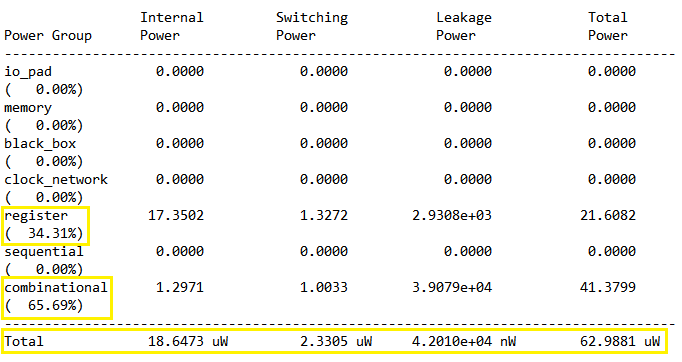
\includegraphics[width=0.8\textwidth]{images/rep_power_x4_mod.png}
	\caption{Power Report}
	\label{fig:pow_rep_x4}
\end{figure}

Si nota come la potenza sia suddivisa tra i registri e la parte combinatoria con una preponderanza di questo secondo contributo, il $65\%$, per via della presenza di 3 moltiplicatori e 2 sommatori nell'architettura progettata.

\subsection{Place \& Route}
Finally si è passati di place and route con l'ausilio del software Innovus. E' stata utilizata la netlist generata da Synopsys con $T_{CLK} = 4 T_{min}$ come punto di partenza e le librerie standard fornite. Dopo le varie fasi richieste si è giunti al circuto finale mostrato in \autoref{fig:layout}.

\begin{figure}[h]
	\center
	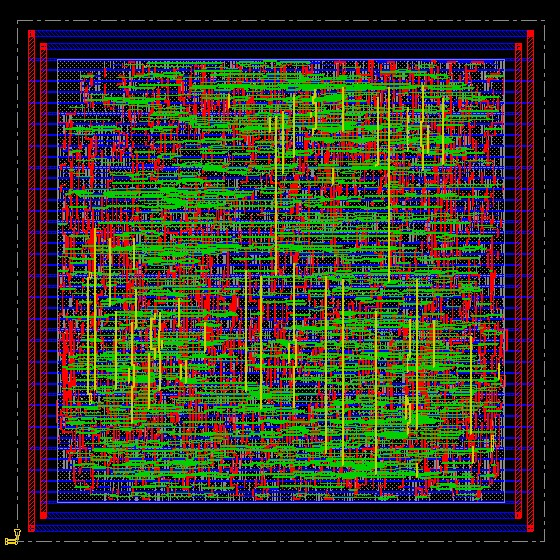
\includegraphics[width=0.6\textwidth]{images/IIR_filter_period_min_x4_place.jpg}
	\caption{Resulting layout}
	\label{fig:layout}
\end{figure}

Il layout prodotto ha un area pari a $\SI{1959}{\micro\meter}^2$, dato concorde con quello stimato da Synopsys mostrato in \autoref{tab:timing_rep}, con un totale di 986 cells and 2455 gates. Succesivamente è stata lanciata la timing analysys per verificare che i timing constraints fossero corretti, con esito positivo. Infine sfruttando la switching activity calcolata con Modelsim è stato stimato nuovamente il consumo di potenza. I risultati ottenuti sono mostrati in \autoref{fig:cadence_pow_rep_x4}.

\begin{figure}[h]
	\center
	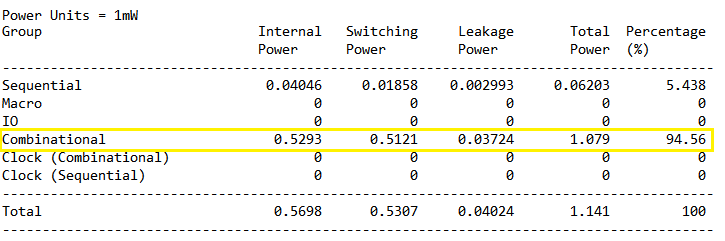
\includegraphics[width=0.8\textwidth]{images/rep_power_x4_cadence_mod.png}
	\caption{Post place \& route power report}
	\label{fig:cadence_pow_rep_x4}
\end{figure}

I valori di potenza ottenuti sono concordi con quelli ottenuti da Synopsys in \autoref{fig:pow_rep_x4}. Inoltre, essendo il calcolo a questo livello molto più accurato in quanto prende in considerazione in layout fisico del circuito, si nota come in realtà il consumo della parte combinatore sia ancora più predominante del previsto. 
